\section{Multi-way Merge Semantic \textsf{ORDER BY}}
\label{sec:framework}

A listwise call can rank at most $m$ items according to the instruction $\phi$. When $n>m$, the operator must combine the orders returned by different calls. We adopt the two phases of external merge sort~\cite{DBLP:journals/csur/Graefe06}: first generate locally sorted runs, then merge them in groups of at most $k$. The physical design question is which rows from a group to put in each prompt. Comparing only the current heads can cost one call per output item; submitting a larger batch can also waste tokens if the same items appear in several prompts.

Figure~\ref{fig:framework} shows how we make this choice. Once the runs are available, the planner uses their lengths, the call capacity $m$, the requested output (Full or \textsf{LIMIT}~$K$), and the input-token profile to select a merge plan. A plan specifies the group-merging algorithm $f$, maximum fan-in $k$, and quota or segment length $h$. We consider two algorithms: sliding window (SW) ranks a window spanning the active runs; segmented loser tree (LT($h$)) ranks the items on one tree path at a time. The planner minimizes estimated \emph{merge input tokens} over the feasible configurations of the requested family, or over both families in automatic mode (Section~\ref{sec:cost}). The executor uses the selected plan to produce either a full order or a prefix.

\begin{figure*}[t]
  \centering
  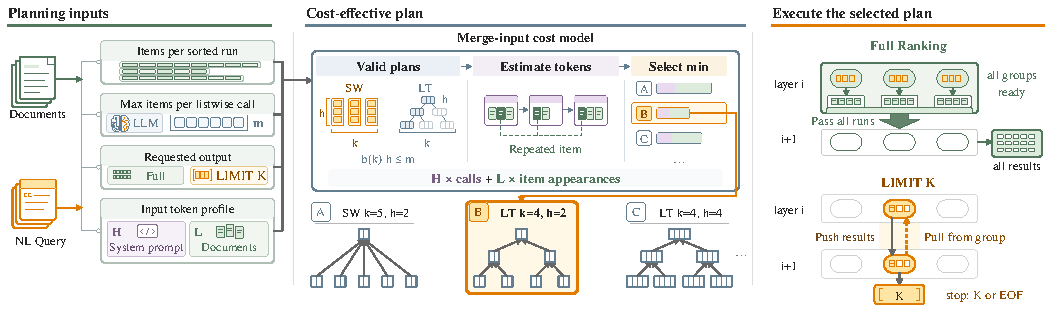
\includegraphics[width=\textwidth]{fig/mechanisms/framework.pdf}
  \caption{Cost-guided semantic \textsf{ORDER BY}. The planner compares feasible merge plans using estimated input tokens. Full ranking materializes layers; \LIMIT~$K$ requests input at group granularity. The candidate plans and token bars are schematic.}
  \label{fig:framework}
\end{figure*}


\subsection{Run Generation and Group Merge}
\label{sec:external-merge}
Algorithm~\ref{alg:semantic_external_merge} implements both phases. It partitions $D$ into $r=\lceil n/m\rceil$ disjoint chunks and ranks each chunk under the same instruction $\phi$. These calls are independent. The resulting sequences $R_1,\ldots,R_r$ are the initial runs. If there is only one run, its first $K$ items (or the whole run for Full) already answer the query.

% Paper abstraction: default no-evidence/no-shuffle path; no execution change.
{\footnotesize\raggedright
\noindent\textit{Conventions.}
$\Rank_\phi(X)$ orders real rows best first; $|X|\le1$ needs no call.
$\operatorname{take}_q$ reads the next $q$ rows or stops at exhaustion ($q=\infty$: drain).
$\Vert$ concatenates in order; $B_u$ is run $u$'s subsequence in $B$.
$\operatorname{unread}(u)$ means unread supply remains.
$\mathcal L(X)$ ranks $X$ once to order the active heads ($\rho$).
$[\bot_a]^r$ means $r$ virtual entries tagged $a$; $\operatorname{real}$ removes them.
$\MergeGroup$ forwards singletons; Full materializes each pass, LIMIT pulls and truncates only the root.
$\mathcal F$ is the feasible set; estimates use run lengths, token profile, mode and $K$.
\textsc{HalvingTree} rounds the left size up; \textsc{Cut} takes maximal subtrees within the frontier bound.\par}


\algcolstart
\begin{algorithm}[H]
\caption{External Merge Group via $k$-Way Merge}
\label{alg:semantic_external_merge}
\KwIn{rows $D$, instruction $\phi$, capacity $m$, mode Full or LIMIT, bound $K$ (default $\infty$)}
\lIf{$D=\varnothing$ or $K=0$}{\Return $[\,]$}
$\mathcal R\leftarrow[\Rank_\phi(C):C\in\operatorname{Chunks}_m(D)]$\;
\lIf{$|\mathcal R|=1$}{\Return $\operatorname{take}_K(\mathcal R_1)$}
$(f,k,h)\leftarrow\arg\min_{(f,k,h)\in\mathcal F}\widehat C_{\rm merge}(f,k,h)$\;
\While{$|\mathcal R|>1$}{
  $\mathcal G\leftarrow\operatorname{Chunks}_k(\mathcal R)$\;
  $\mathcal R'\leftarrow[\MergeGroup_{f,h}(G):G\in\mathcal G]$\;
  \lIf{Full}{$\mathcal R'\leftarrow[\operatorname{materialize}(S):S\in\mathcal R']$}
  $\mathcal R\leftarrow\mathcal R'$\;
}
\Return $\operatorname{take}_K(\mathcal R_1)$\;
\end{algorithm}
\algcolend


For multiple runs, the algorithm selects the plan once and partitions the current runs into consecutive groups of at most $k$ in each pass. Each invocation of \textsc{MergeGroup} combines one group into a run; a singleton passes through unchanged. In Full mode, groups in the same pass can execute in parallel. The next pass begins once their outputs have been materialized. Figure~\ref{fig:alg1-full-trace} illustrates this schedule for $n=16$, $m=4$, and $k=2$. Four listwise calls generate four runs. The first merge pass combines $R_1$ with $R_2$ and $R_3$ with $R_4$; the second merges the two outputs. A group merge can require several listwise calls, as the following algorithms show.

\begin{figure}\centering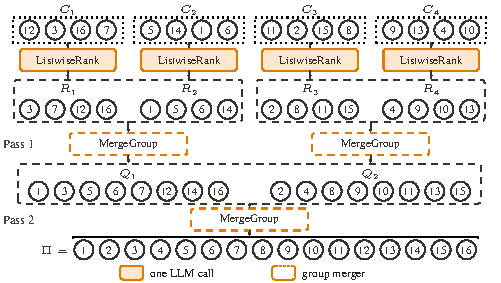
\includegraphics[width=\columnwidth]{fig/mechanisms/alg1-trace/alg1-trace.pdf}\caption{Algorithm 1, Full trace ($n=16$, $m=4$, fixed $k=2$). Four listwise calls generate runs; two merge passes reduce $4\to2\to1$ runs. MergeGroup uses SW or LT($h$) and may make multiple calls.}\label{fig:alg1-full-trace}\end{figure}


\subsection{Sliding-Window Merge}
\label{sec:sw}
SW amortizes one call over several output items by taking a short prefix from \emph{each} active run. Algorithm~\ref{alg:sliding_window_kway_group_merge} retains un-emitted items in a buffer $B$. Let $A$ contain the runs with items in $B$ or with unread input. The optimized SW plan fixes the integer quota $h$ for both Full and \textsf{LIMIT}. It refills only each run's deficit up to $h$ and leaves slots vacant when the run has too few items. When only one run remains, SW forwards its remaining items in run order without another call.

\algcolstart
\begin{algorithm}[H]
\caption{Sliding-Window Semantic $k$-Way Merge}
\label{alg:sliding_window_kway_group_merge}
\KwIn{$2\le g\le m$ runs; quota $1\le h\le\lfloor m/g\rfloor$}
$B\leftarrow[\,]$\;
\While{$B\ne[\,]$ or some run is unread}{
  $A\leftarrow\{u:|B_u|>0\ \lor\ \operatorname{unread}(u)\}$\;
  \ForEach{$u\in A$ in run order}{
    $B\leftarrow B\Vert\operatorname{take}_{\max(0,h-|B_u|)}(R_u)$\;
  }
  \lIf{$B=[\,]$}{stop}
  $A\leftarrow\{u:|B_u|>0\ \lor\ \operatorname{unread}(u)\}$\;
  \lIf{$A=\{u\}$}{yield $B_u$ then stream $R_u$ on demand; stop}
  $O\leftarrow\Rank_\phi(B)$\;
  $J\leftarrow\{j:\exists u,\ \operatorname{unread}(u),\ |B_u|>0,$\;
  \Indp $\qquad |(O_{1:j})_u|=|B_u|\}$\;\Indm
  $t\leftarrow\min(J\cup\{|O|\})$\;
  yield $O_{1:t}$; $B\leftarrow\operatorname{stableRemove}(B,O_{1:t})$\;
}
\end{algorithm}
\algcolend


\paragraph{Where to stop.}
Let $O$ be the listwise ranking of $B$. SW scans $O$ in order and emits through the first item that empties the buffered portion of a run \emph{with unread input}. The next item of that run was absent from the call and could precede the rest of $O$. A run with no unread input imposes no such boundary. If no run imposes a boundary, SW emits all of $O$. Under a common ordering of the runs and the batch, every emitted item precedes the unseen suffixes: until the boundary, each nonempty unseen suffix still has a buffered predecessor, including the boundary item itself for the run that triggers the stop. This is the sense in which the prefix is \emph{safe} (Appendix~\ref{app:proof-sw}). SW removes the emitted items from $B$, preserving the buffer order of the survivors for the next refill.

\begin{figure}[t]
  \centering
  % SVG physical metrics target this measured VLDB column width.
  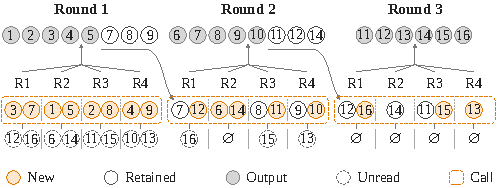
\includegraphics[width=\linewidth]{fig/mechanisms/sw.pdf}
  \caption{Sliding-window merge ($m=8$), emitting $5+5+6$ items. A prefix ends when a run with unread rows empties its window: $R_2$ at 5, then $R_4$ at 10. With nothing unread, round 3 drains the buffer. Retained items stay buffered without reordering; windows are grouped by run for display.}
  \label{fig:sw-mechanism}
\end{figure}


In Figure~\ref{fig:sw-mechanism}, four runs contribute two items each to a window of size eight. The first call places $1,2,3,4,5$ first. Item~5 consumes the last buffered item of $R_2$, but $R_2$ still holds~6. Emitting~7 from the same ranking would therefore skip~6. The second call includes~6 and emits through~10, where $R_4$ must be refilled. In the third call no run has unread input, so the remaining six items are all emitted.

\subsection{Segmented Loser-Tree Merge}
\label{sec:lt}
When SW refills even one run, it resubmits the surviving items from the whole window. LT($h$) confines each update to one path through a binary tree. Its leaves represent the $g$ runs of the group. Each internal node retains a \emph{loser segment} of at most $h$ rows and a pointer to one child. A \emph{winner segment} travels upward; at the root it becomes the next output. No other winner segments need to persist between refreshes.

\algcolstart
\begin{algorithm}[H]
\caption{Loser-Tree Semantic $k$-Way Merge}
\label{alg:loser_tree_kway_group_merge}
\KwIn{$g\ge2$ runs, $h\ge1$, $(1+\lceil\log_2 g\rceil)h\le m$}
$T\leftarrow\operatorname{HalvingTree}(R_1,\ldots,R_g)$; $F\leftarrow\operatorname{leaves}(T)$\;
\ForEach{$u\in F$}{$S_u\leftarrow\operatorname{take}_h(R_u)$}
\While{$F\ne\{\mathrm{root}\}$}{
  $\mathcal B\leftarrow\operatorname{Cut}(T,F,\lfloor m/h\rfloor)$\;
  \ForEach{$b\in\mathcal B$ with more than one frontier leaf}{
    $X\leftarrow\mathop{\Vert}_{u\in F\cap b}^{\rm left\ to\ right}S_u$;
    $\rho\leftarrow\mathcal L(X)$\;
    \ForEach{new internal $v$ of $b$, bottom-up}{
      $(S_v,\ell_v,p_v)\leftarrow\Replay(v,S_{v_L},S_{v_R},\rho)$\;
    }
  }
  $F\leftarrow\{\operatorname{root}(b):b\in\mathcal B\}$\;
}
\While{$S_{\rm root}\ne[\,]$}{yield $S_{\rm root}$; $S_{\rm root}\leftarrow\Refresh(T)$}
\end{algorithm}
\algcolend


\paragraph{Building the tree.}
Algorithm~\ref{alg:loser_tree_kway_group_merge} recursively halves the runs, giving the larger half to the left child when the count is odd. The resulting tree has exactly $g$ leaves and depth $d=\lceil\log_2 g\rceil$. Each leaf initially supplies up to $h$ items. If all $gh$ slots fit in a prompt, a single rank map suffices for bottom-up construction. Otherwise, the algorithm partitions the current frontier into maximal subtrees with at most $\lfloor m/h\rfloor$ frontier segments each. For each such subtree it ranks the real rows together, replays its internal matches using that rank map, and takes the subtree winner as one segment of the next frontier. This repeats until the root winner is available. To form a rank map $\rho$, LT preserves each input run's established order: among eligible run heads it repeatedly takes the head ranked earliest in the listwise response.

\begin{figure}[t]
  \centering
  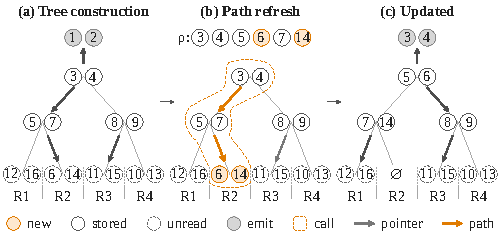
\includegraphics[width=\linewidth]{fig/mechanisms/lt.pdf}
  \caption{A refresh in a segmented loser tree ($h=2$). After the root emits $[1,2]$, the pointers lead to $R_2$. The ranker sees the replacement segment and only the losers on that path. Replaying the two matches yields $[3,4]$.}
  \label{fig:lt-mechanism}
\end{figure}


\paragraph{Choosing the next child.}
A winner segment can contain items from both children. The origin of its last item therefore does not tell us which child to refill. Algorithm~\ref{alg:replay_segment_node} makes two distinct decisions from the same ranking. It tags the two input segments as left and right \emph{slots} and orders their rows by $\rho$. The first $h$ positions supply the winner, and the remainder form the stored loser. To set the pointer, it scans the entire ranked sequence until either slot contributes its $h$-th entry. The child corresponding to that slot is the one whose next segment is needed. At a run tail, virtual entries complete each slot to length $h$ after the real rows; they affect the slot counts but never enter a prompt or an output.

\algcolstart
\begin{algorithm}[H]
\caption{Node Replay}
\label{alg:replay_segment_node}
\KwIn{node $v$, slots $s_L,s_R$ with $|s_L|,|s_R|\le h$, rank map $\rho$}
$Z\leftarrow\operatorname{sort}_\rho(s_L\Vert s_R)$, retaining slot tags\;
$Z\leftarrow Z\Vert[\bot_L]^{h-|s_L|}\Vert[\bot_R]^{h-|s_R|}$\;
$j^*\leftarrow\min\{j:\max_{a\in\{L,R\}}|(Z_{1:j})_a|=h\}$\;
$p\leftarrow v_{\operatorname{slot}(Z_{j^*})}$\;
\Return $(\operatorname{real}(Z_{1:h}),\operatorname{real}(Z_{h+1:}),p)$\;
\end{algorithm}
\algcolend

\begin{figure}[t]
  \centering
  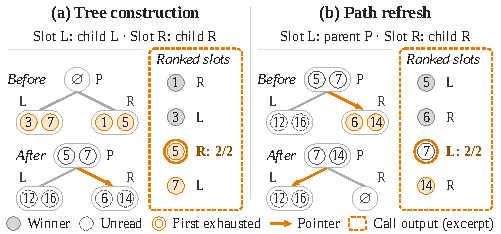
\includegraphics[width=\linewidth]{fig/mechanisms/pointer.pdf}
  \caption{Pointer assignment ($h=2$). The first slot to supply its second entry in the replay order determines the pointer. In (a), R reaches that entry at row 5. In (b), the old parent segment occupies L and reaches its second entry at row 7. L and R are slot labels, not the original run identities.}
  \label{fig:pointer-mechanism}
\end{figure}


Figure~\ref{fig:pointer-mechanism}(a) illustrates the distinction for $h=2$. The ranked slots are $1_R,3_L,5_R,7_L$. The winner is $[1,3]$, but the pointer selects the right child: its second entry is~5, before the left slot's second entry~7. The node retains $[5,7]$. These rows came from different children; at the next replay they occupy one slot together. In Figure~\ref{fig:pointer-mechanism}(b), that retained segment occupies the left slot and the incoming $[6,14]$ occupies the right. The node forwards $[5,6]$, keeps $[7,14]$, and now points left.

\paragraph{Refreshing one path.}
After the root segment has been emitted, Algorithm~\ref{alg:refresh_loser_tree_path} follows child pointers from the root to one leaf. It pulls that run's next segment and collects the loser segments stored on the path. A single listwise call ranks the collected real rows when at least two are present. The path contains at most $d$ internal nodes, so the prompt contains at most $(d+1)h$ items; this is why LT requires $(d+1)h\le m$. The algorithm replays the path bottom-up under the resulting $\rho$. At each node, the incoming segment occupies the slot named by the old pointer, and the previously stored loser occupies the other slot. Replay installs the new loser and pointer and sends the winner upward. All nodes outside the path keep their state. Even when calls disagree, this replay rule preserves the order of each input run and emits only prefixes of it (Appendix~\ref{app:proof-inconsistent}).

\algcolstart
\begin{algorithm}[H]
\caption{Path Refresh}
\label{alg:refresh_loser_tree_path}
\KwIn{LT($h$) $T$ after root emission; losers $\ell_v$ and child pointers $p_v$ at internal nodes}
$P\leftarrow[\,]$; $u\leftarrow\operatorname{root}(T)$\;
\While{$u$ is internal}{$P\leftarrow P\Vert[u]$; $u\leftarrow p_u$}
$S\leftarrow\operatorname{take}_h(R_u)$\;
$X\leftarrow S\Vert\mathop{\Vert}_{v\in P}\ell_v$; $\rho\leftarrow\mathcal L(X)$\;
\ForEach{$v\in\operatorname{reverse}(P)$}{
  $(s_L,s_R)\leftarrow(S,\ell_v)$ if $p_v=v_L$, else $(\ell_v,S)$\;
  $(S,\ell_v,p_v)\leftarrow\Replay(v,s_L,s_R,\rho)$\;
}
\Return $S$\;
\end{algorithm}
\algcolend


Figure~\ref{fig:lt-mechanism} traces one refresh on the same four runs as SW, with $h=2$. After the root emits $[1,2]$, the pointers lead to $R_2$. Its new segment $[6,14]$ joins $[5,7]$ and $[3,4]$, the two stored losers on the path. The repaired rank map orders these six rows as $[3,4,5,6,7,14]$. Two local replays produce the next root segment $[3,4]$ without another model call. The right subtree, which retains $[8,9]$, contributes no rows to this prompt.

\paragraph{The single-item case.}
Setting $h=1$ recovers the structure of the classical loser tree~\cite{DBLP:journals/csur/Graefe06}. Each node stores one loser, each nonempty root segment contains one winner, and the pointer follows the child supplying that winner. Refresh replaces one run head and replays its path. The semantic implementation still ranks the replacement and its path opponents together; the binary matches use positions in that ranking. Increasing $h$ uses the same tree and replay rule to deliver up to $h$ items per refresh.

\subsection{Demand-Driven Execution for \textsf{LIMIT}~$K$}
\label{sec:topk}\label{sec:topk-exec}
Materializing every group would compute intermediate tails that a prefix query might never read. For a prefix in the ranker's output direction, we keep run generation unchanged and execute the merge groups as producers. A leaf serves an initial run in order. An internal producer answers a request for rows first from its pending output; when it needs more, it advances its own merger. In strict-demand mode there is no background prefetch. An SW group pulls enough from each deficient child to form its window. An LT group initially pulls a segment from each child and subsequently refills only the leaf named by its pointer path. A request for even one output row can thus require several child rows or a complete listwise call. The limit applies to rows returned by the root, not to the number of rows that each child may supply.

The root stops after $K$ items or on exhaustion, and the executor closes the producer tree. It does not start a new root refresh to complete a segment after meeting the limit. For example, with $K=3$ in Figure~\ref{fig:lt-mechanism}, the root returns the initial $[1,2]$ and the first item of the next segment $[3,4]$. It then stops without following another pointer. For a fixed merge plan and identical listwise responses on the calls it reaches, this returns the prefix of the full execution of \emph{that plan}: each group consumes the same child prefixes and performs the same state transitions until the final requested item. This execution saves work on intermediate tails; we next estimate how much of that work each candidate plan avoids.
